%%%%%%%%%%%%%%%%%%%%%%%%%%%%%%%%%%%%%%%%%
% Jacobs Landscape Poster
% LaTeX Template
% Version 1.0 (29/03/13)
%
% Created by:
% Computational Physics and Biophysics Group, Jacobs University
% https://teamwork.jacobs-university.de:8443/confluence/display/CoPandBiG/LaTeX+Poster
% 
% Further modified by:
% Nathaniel Johnston (nathaniel@njohnston.ca)
%
% This template has been downloaded from:
% http://www.LaTeXTemplates.com
%
% License:
% CC BY-NC-SA 3.0 (http://creativecommons.org/licenses/by-nc-sa/3.0/)
%
%%%%%%%%%%%%%%%%%%%%%%%%%%%%%%%%%%%%%%%%%

%----------------------------------------------------------------------------------------
%	PACKAGES AND OTHER DOCUMENT CONFIGURATIONS
%----------------------------------------------------------------------------------------
\documentclass[12pt]{beamer}

\usepackage[scale=1.24]{beamerposter} % Use the beamerposter package for laying out the poster
\usepackage{graphicx} % more modern 
\usepackage{caption}
\usepackage{subcaption}
\usepackage{tikz}
\usepackage{dsfont}
\usepackage{amsmath}
\usepackage{amssymb}
\usepackage{amsthm}
\usepackage{times}
\usepackage{natbib}
\usepackage{xcolor}
\usepackage[noend]{algorithmic}
%\algrenewcommand\algorithmicindent{2.0em}%
\algsetup{indent=4em}
\usepackage{algorithm}

\usetheme{confposter} % Use the confposter theme supplied with this template

\setbeamercolor{block title}{fg=ngreen,bg=white} % Colors of the block titles
\setbeamercolor{block body}{fg=black,bg=white} % Colors of the body of blocks
\setbeamercolor{block alerted title}{fg=white,bg=dblue!70} % Colors of the highlighted block titles
\setbeamercolor{block alerted body}{fg=black,bg=dblue!10} % Colors of the body of highlighted blocks
% Many more colors are available for use in beamerthemeconfposter.sty

%-----------------------------------------------------------
% Define the column widths and overall poster size
% To set effective sepwid, onecolwid and twocolwid values, first choose how many columns you want and how much separation you want between columns
% In this template, the separation width chosen is 0.024 of the paper width and a 4-column layout
% onecolwid should therefore be (1-(# of columns+1)*sepwid)/# of columns e.g. (1-(4+1)*0.024)/4 = 0.22
% Set twocolwid to be (2*onecolwid)+sepwid = 0.464
% Set threecolwid to be (3*onecolwid)+2*sepwid = 0.708

\newlength{\sepwid}
\newlength{\onecolwid}
\newlength{\twocolwid}
\newlength{\threecolwid}
\setlength{\paperwidth}{48in} % A0 width: 46.8in
\setlength{\paperheight}{36in} % A0 height: 33.1in
\setlength{\sepwid}{0.024\paperwidth} % Separation width (white space) between columns
\setlength{\onecolwid}{0.22\paperwidth} % Width of one column
\setlength{\twocolwid}{0.464\paperwidth} % Width of two columns
\setlength{\threecolwid}{0.708\paperwidth} % Width of three columns
\setlength{\topmargin}{-0.5in} % Reduce the top margin size
%-----------------------------------------------------------

\usepackage{graphicx}  % Required for including images

\usepackage{booktabs} % Top and bottom rules for tables



\newcommand{\defined}{\vcentcolon =}
\newcommand{\rdefined}{=\vcentcolon}
\newcommand{\E}[1]{\mathbb E\left[#1\right]}
\newcommand{\R}{\mathbb R}
\newcommand{\Var}{\operatorname{Var}}
\newcommand{\calF}{\mathcal F}
\newcommand{\sr}[1]{\stackrel{#1}}
\newcommand{\set}[1]{\left\{#1\right\}}
\newcommand{\ind}[1]{\mathds{1}\!\!\set{#1}}
%\newcommand{\ind}[1]{\set{#1}}
\newcommand{\argmax}{\operatornamewithlimits{arg\,max}}
\newcommand{\argmin}{\operatornamewithlimits{arg\,min}}
\newcommand{\floor}[1]{\left \lfloor {#1} \right\rfloor}
\newcommand{\ceil}[1]{\left \lceil {#1} \right\rceil}
\newcommand{\eqn}[1]{\begin{align}#1\end{align}}
\newcommand{\eq}[1]{\begin{align*}#1\end{align*}}
\newcommand{\Ber}{\operatorname{Bernoulli}}
\renewcommand{\P}[1]{\operatorname{P}\left\{#1\right\}}
\newcommand{\Pri}[1]{\operatorname{P}_i\left\{#1\right\}}
\newcommand{\Prz}[1]{\operatorname{P}_0\left\{#1\right\}}
\newcommand{\bigo}[1]{\mathcal{O}\left( #1 \right)}
\newcommand{\bigotilde}[1]{\tilde{\mathcal{O}}\left( #1 \right)}
\newcommand{\bigtheta}[1]{\Theta\left( #1 \right)}
\newcommand{\bigthetatilde}[1]{\tilde{\Theta}\left( #1 \right)}
\newcommand{\bigomega}[1]{\Omega\left( #1 \right)}
\newcommand{\KL}{\operatorname{KL}}
\newcommand{\simpleregret}{R_T}
\newcommand{\Pij}[1]{\operatorname{P}_{ij}\!\left\{#1\right\}}
\newcommand{\Pkl}[1]{\operatorname{P}_{kl}\!\left\{#1\right\}}
\newcommand{\Q}[1]{\operatorname{Q}\left\{#1\right\}}
\newcommand{\EE}{\mathbb E}
\newcommand{\EEa}{\EE_a}
\newcommand{\Pns}[2]{\operatorname{P}_{#1}\left\{#2\right\}}
\newcommand{\Pn}[2]{\operatorname{P}\left\{#2|#1\right\}}
\newcommand{\parents}[1]{\operatorname{\mathcal{P}a}_{#1}}
\newcommand{\actions}{\mathcal{A}}
\newcommand{\calA}{\mathcal A}
\newcommand{\etc}{\textit{etc}}
\newcommand{\ie}{\textit{i.e.}}
\newcommand{\eg}{\textit{e.g.}}
\newcommand{\calP}{\mathcal P}
\newcommand{\x}{\boldsymbol{x}}
\newcommand{\Ps}{\operatorname{P}}


\let\temp\epsilon
\let\epsilon\varepsilon
\let\vec\mathbf

\graphicspath{ {figures/} }
\usetikzlibrary{arrows,positioning,backgrounds} 
\tikzset{
    %Define standard arrow tip
    >=stealth',
    %Define style for boxes
    observed/.style={
           circle,
           rounded corners,
           draw=black, thick,
           minimum width=2.0em,
           minimum height=2.0em,
           font=\tiny,
           text centered,
           scale=.8,
           fill=blue!20!white},
     latent/.style={
           circle,
           rounded corners,
           draw=black, thick, dashed,
           minimum width=.5em,
           minimum height=.5em,
           font=\footnotesize,
           text centered,
           fill=black!10!white
           },
     empty/.style={
           circle,
           rounded corners,
           minimum width=.5em,
           minimum height=.5em,
           font=\footnotesize,
           text centered,
           },
    % Define arrow style
    pil/.style={
           o->,
           thick,
           shorten <=2pt,
           shorten >=2pt,},
    sh/.style={ shade, shading=axis, left color=red, right color=green,
    shading angle=45 }  
}

%----------------------------------------------------------------------------------------
%	TITLE SECTION 
%----------------------------------------------------------------------------------------

\title{Causal Bandits: Learning Good Interventions via Causal Inference} % Poster title

\author{Finnian Lattimore*, Tor Lattimore** and Mark Reid*} % Author(s)

\institute{*Australian National University and Data61, **University of Indiana Bloomington} % Institution(s)

%----------------------------------------------------------------------------------------

\begin{document}

\addtobeamertemplate{block end}{}{\vspace*{2ex}} % White space under blocks
\addtobeamertemplate{block alerted end}{}{\vspace*{2ex}} % White space under highlighted (alert) blocks

\setlength{\belowcaptionskip}{2ex} % White space under figures
\setlength\belowdisplayshortskip{2ex} % White space under equations

\begin{frame}[t] % The whole poster is enclosed in one beamer frame

\begin{columns}[t] % The whole poster consists of three major columns, the second of which is split into two columns twice - the [t] option aligns each column's content to the top

\begin{column}{\sepwid}\end{column} % Empty spacer column

\begin{column}{\onecolwid} % The first column

%----------------------------------------------------------------------------------------
%	OBJECTIVES
%----------------------------------------------------------------------------------------

%\begin{alertblock}{Objectives}
%
%Lorem ipsum dolor sit amet, consectetur, nunc tellus pulvinar tortor, commodo eleifend risus arcu sed odio:
%\begin{itemize}
%\item Mollis dignissim, magna augue tincidunt dolor, interdum vestibulum urna
%\item Sed aliquet luctus lectus, eget aliquet leo ullamcorper consequat. Vivamus eros sem, iaculis ut euismod non, sollicitudin vel orci.
%\item Nascetur ridiculus mus.  
%\item Euismod non erat. Nam ultricies pellentesque nunc, ultrices volutpat nisl ultrices a.
%\end{itemize}
%
%\end{alertblock}

%----------------------------------------------------------------------------------------
%	INTRODUCTION
%----------------------------------------------------------------------------------------

\begin{block}{Introduction}

We study the problem of using causal models to improve the rate at which good interventions can be learned online in a stochastic environment. 
Our formalism combines multi-arm bandits and causal inference to model a novel type of bandit feedback that is not exploited by existing approaches.
We propose a new algorithm that exploits the causal feedback and prove a bound on its simple regret that is strictly better (in all quantities) 
than algorithms that do not use the additional causal information.

\end{block}

%------------------------------------------------
\begin{block}{Setup}
\begin{itemize}
\item Learner given causal graph $\mathcal{G}$ over a set of random variables $\mathcal{X}$
\item Actions assign values to subsets of variables in $\mathcal{G}$. The set of allowed actions/arms $\mathcal{A}$ is a subset of all possible assignments.
\item One variable $Y \in \mathcal{X}$ is designated as the \emph{reward variable} and takes on values in $\{0, 1\}$.
\item The game proceeds over $T$ rounds. In round $t$, the learner takes action $a_t = do(\vec{X}_t = \vec{x}_t) \in \mathcal{A}$, \textbf{\emph{then}} observes reward $Y_t$ and the value of all other variables in $\mathcal{X}$.
\item Simple regret: goal is to minimize $\simpleregret = \mu^* - \E{\mu_{\hat a^*_T}}$, where $\mu^*$ is the expected reward of the best action and $\hat a^*_T$ is the action the learner estimates to be optimal at time $T$
\end{itemize}


\begin{figure}
    \begin{subfigure}[b]{0.45\textwidth}
	\centering    
          \begin{tikzpicture}[->,>=stealth',shorten >=1pt,auto,node distance=1.0em,
  thick,main node/.style={observed}, hidden/.style={empty},background rectangle/.style={fill=olive!45}]
%every node/.style={scale=0.6}
 %nodes
\node[main node](1){$X_{1}$};
\node[main node, right=of 1](2){$X_{2}$};
\node[hidden, right=of 2](3){$...$};
\node[main node, right=of 3](4){$X_{N}$};
\node[main node, below right=of 2](5){$Y$};
 \path[every node/.style={font=\tiny}]
    (1) edge (5)
    	(2) edge (5)
    (4) edge (5);
\end{tikzpicture}
        \caption{Parallel graph}
        \label{fig:parallel}
    \end{subfigure}
    \begin{subfigure}[b]{0.5\textwidth}
    \centering    
          \begin{tikzpicture}[->,>=stealth',shorten >=1pt,auto,node distance=1.0em,
  thick,main node/.style={observed}, hidden/.style={empty},background rectangle/.style={fill=olive!45}]
%every node/.style={scale=0.6}
 %nodes
\node[main node](1){$X_{1}$};
\node[main node, right=of 1](2){$X_{2}$};
\node[hidden, right=of 2](3){$...$};
\node[main node, right=of 3](4){$X_{N}$};
\node[main node, below right=of 2](5){$Y$};
\node[main node, above right=of 2](6){$Z$};
 \path[every node/.style={font=\tiny}]
    (1) edge (5)
    	(2) edge (5)
    (4) edge (5)
    (6) edge (1) edge (2) edge (4);
\end{tikzpicture}
        \caption{Confounded parallel graph}
        \label{fig:parallel_confounded} 
    \end{subfigure} 
\caption{Causal graphs}
\label{fig:causal graphs} 
\end{figure}

\end{block}

\begin{block}{Parallel Model}

\begin{itemize}
\item Causal graph as in figure \ref{fig:parallel} with all variables binary.
\item $\mathcal{A} = \set{do()} \cup \set{ do(X_i = j) \colon 1 \leq i \leq N \text{ and } j \in \set{0,1}}$
\item For this causal model, $P(Y|do(X_i = j)) = P(Y|X_i = j)$
\item $\vec{q} = (q_1, \ldots, q_N) \in [0,1]^N$ so that $q_i = \P{X_i = 1}$
\item $I_\tau = \set{ i : \min\set{q_i, 1-q_i} < \frac{1}{\tau}}$ is set of 'unbalanced' variables using a threshold $1/\tau$
\item The difficulty of the problem is captured by:
\eq{
\label{eq:m-simple}
m(\vec{q}) = \min \set{ \tau : |I_{\tau}| \leq \tau}\,.
}
\end{itemize} 




\end{block}
\end{column} % End of the first column


%----------------------------------------------------------------------------------------
\begin{column}{\onecolwid} % The 2nd
\begin{block}{Parallel Algorithm}
\setbeamercolor*{block body}{bg=white!95!blue,fg=black}
\begin{algorithm}[H]
\caption{ Parallel Bandit Algorithm \textcolor{white}{\Large A}}\label{alg:simple}
\begin{algorithmic}[1]
\STATE {\bf Input:} Total rounds $T$ and $N$.
\FOR{$t \in 1,\ldots,T / 2$}
\STATE Perform empty intervention $do()$
\STATE Observe $\vec{X}_t$ and $Y_t$
\ENDFOR
\FOR{$a = do(X_i = x) \in \actions$}
\STATE Count times $X_i = x$ seen: $T_a = \sum_{t=1}^{T/2} \ind{X_{t,i} = x}$
\STATE Estimate reward: $\hat{\mu}_a = \frac{1}{T_a} \sum_{t=1}^{T/2} \ind{X_{t,i} = x} Y_t$ \\[0.2cm]
\STATE Estimate probabilities: $\hat{p}_a = \frac{2 T_a}{T}$,\,\, $\hat q_i = \hat p_{do(X_i = 1)}$
\ENDFOR
\STATE Compute $\hat{m} = m(\vec{\hat q})$ and $A = \set{a \in \actions \colon \hat{p}_a \leq \frac{1}{\hat m}}$.
\STATE Let $T_A := \frac{T}{2 |A|}$ be times to sample each $a\in A$.
\FOR{$a = do(X_i = x) \in A$}
\FOR{$t \in 1,\ldots,T_A$}
\STATE Intervene with $a$ and observe $Y_t$
\ENDFOR
\STATE Re-estimate $\hat{\mu}_a = \frac{1}{T_A} \sum_{t=1}^{T_A} Y_t$
\ENDFOR
\RETURN estimated optimal $\hat{a}^*_T \in \argmax_{a\in\actions} \hat{\mu}_a$
\end{algorithmic}
\end{algorithm}

\eq{
&\textbf{upper-bound, } \simpleregret \in \bigo{\sqrt{\frac{m(\vec{q})}{T}\log\left(\frac{NT}{m(\vec{q})}\right)}}\,.\\
&\textbf{lower-bound, }\simpleregret \in \Omega\left(\sqrt{\frac{m(\vec{q})}{T}}\right)\,.\\
&\textbf{standard lower-bound, }\simpleregret \in \Omega\left(\sqrt{\frac{N}{T}}\right)\,.
}

\end{block}

\begin{block}{General Graphs}
\begin{itemize}
\item Known but arbitrary causal structure.
\item It's no longer optimal to split between $do()$ and explicitly playing actions. 
\item We assume the conditional interventional distributions over the parents of $Y$, $\P{\parents{Y}|a}$, are known.
\item $\eta$ is a distribution on available interventions that allocates samples to actions.
\item We use a (truncated) importance weighted estimator to transfer information across different actions. 
\item The (untruncated) weights for each action, $R_a(X,\eta) = \frac{\Pn{a}{\parents{Y}(X)}}{ \sum_{a \in \calA} \eta_a \P{\parents{Y}|a}}$, depend on how different the distribution of the parents of $Y$ is under $a$ to the distribution given actions sampled from $\eta$.
\item We optimise $\eta$ to minimize the simple regret.
\eq {
\eta^*  = \argmin_\eta \underbrace{\max_{a \in \calA} \EEa \left[R_a(X,\eta)\right]}_{m(\eta)}\,.
} 
\item The difficulty of the problem is captured by $m(\eta*)$

\end{itemize}
\end{block}
\end{column}


\begin{column}{\onecolwid} % The 2nd
\begin{block}{General Algorithm}
\begin{algorithm}[H]
\caption{General Algorithm  \textcolor{white}{\Large A}}\label{alg:general}
\begin{algorithmic}
\STATE {\bf Input:} $T$, $\eta \in [0,1]^{\calA}$, $B \in [0,\infty)^{\calA}$
\FOR{$t \in \set{1,\ldots,T}$}
\STATE Sample action $a_t$ from $\eta$
\STATE Do action $a_t$ and observe $X_t$ and $Y_t$
\ENDFOR
\FOR{$a \in \calA$}
\STATE
\eq {
\hat \mu_a =  \frac{1}{T} \sum_{t=1}^T Y_t R_a(X_t,\eta)  \ind{R_a(X_t,\eta) \leq B_a}
}
\ENDFOR
\STATE {\bf return} $\hat a^*_T = \argmax_a \hat \mu_a$
\end{algorithmic}
\end{algorithm}

\eq{
\textbf{upper-bound, } \simpleregret \in \bigo{\sqrt{\frac{m(\eta)}{T} \log\left(2NT\right)}}\,.
}



\end{block}

\begin{block}{Experiments}
\begin{figure}
    \begin{subfigure}[t]{0.3\textwidth}
		\centering    
    		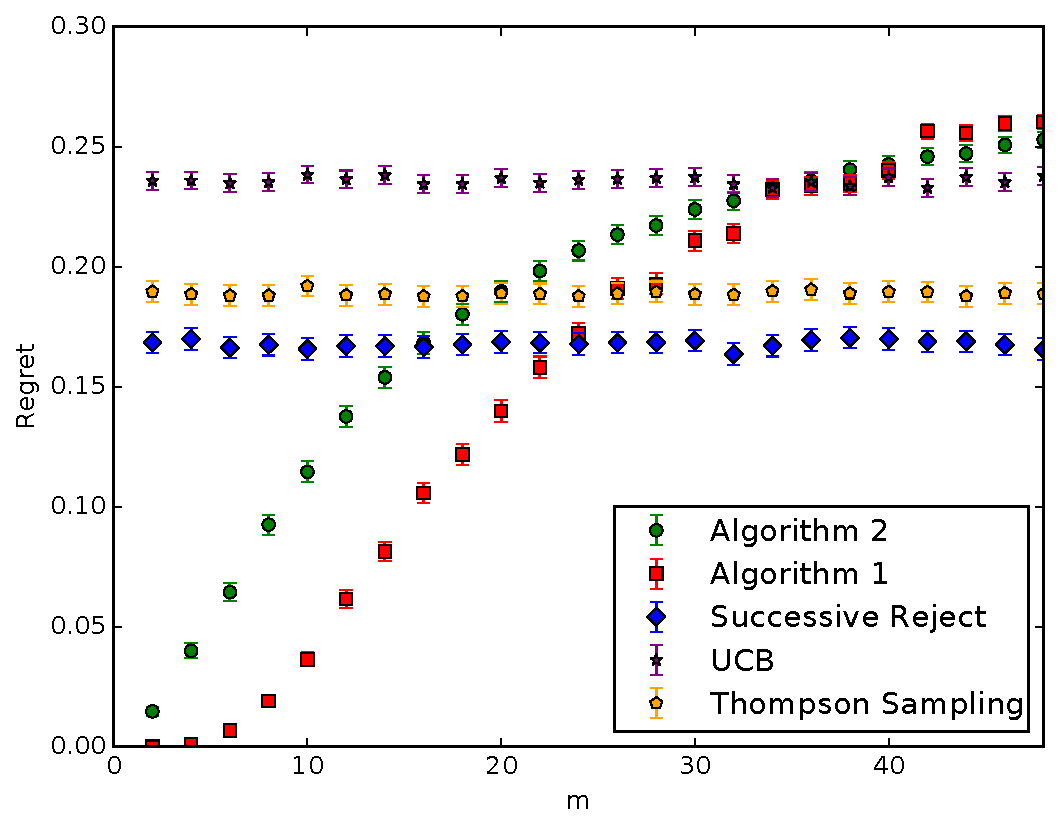
\includegraphics[width=\textwidth]{experiment1_20161020_1247.pdf}
    		\caption{Simple regret vs $m(\boldsymbol{q})$ for fixed horizon $T=400$ and number of variables $N = 50$}
        \label{fig:simple_vs_m}
    \end{subfigure}\hfill
    \begin{subfigure}[t]{0.3\textwidth}
    		\centering
        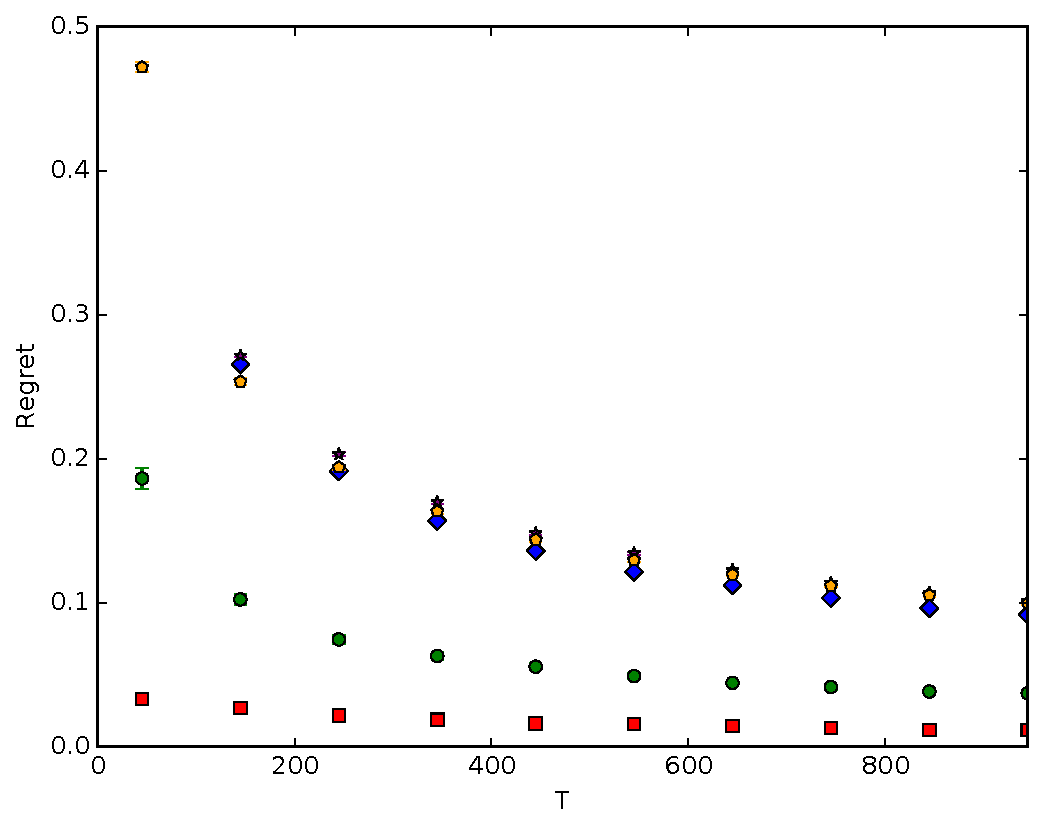
\includegraphics[width=\textwidth]{experiment2_20161020_1249.pdf}
    		\caption{Simple regret vs horizon, $T$, with $N = 50$, $m=2$ and $\epsilon = \sqrt{\frac{N}{8T}}$}
        \label{fig:simple_vs_T_vary_epsilon}
    \end{subfigure}\hfill
    \begin{subfigure}[t]{0.3\textwidth}
    		\centering
    		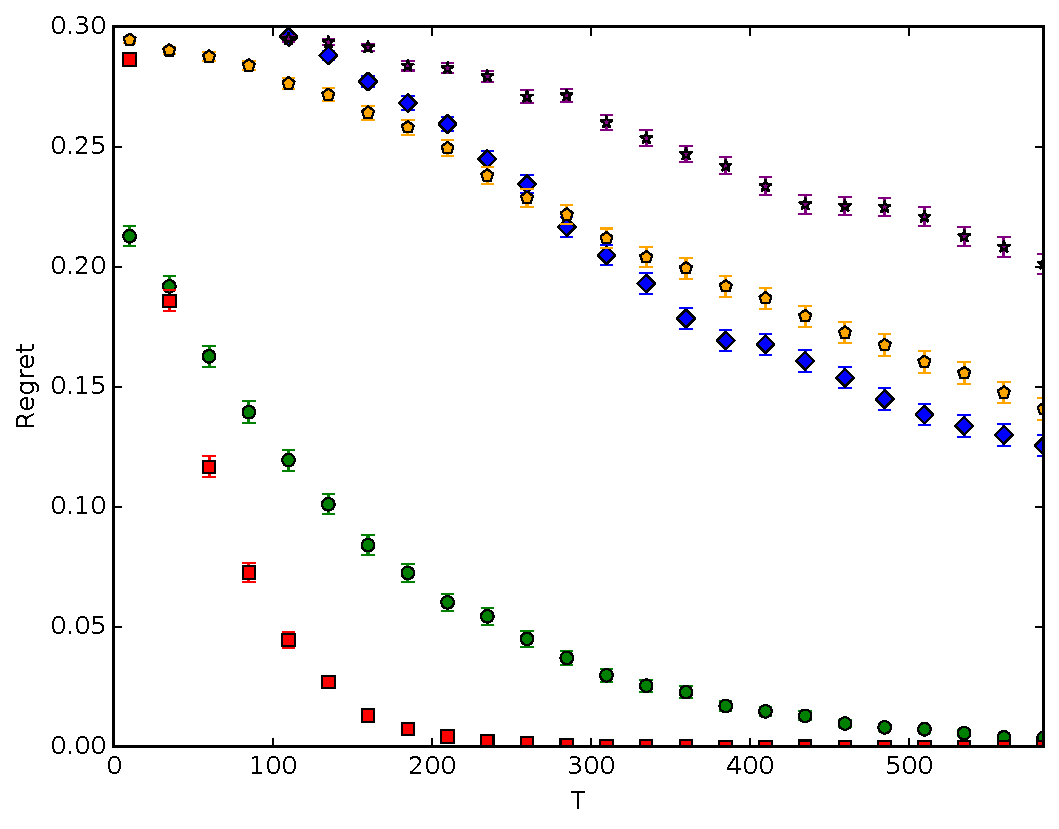
\includegraphics[width=\textwidth]{experiment3_20161020_1252.pdf}
    		\caption{Simple regret vs horizon, $T$, with $N = 50$, $m=2$ and fixed $\epsilon = .3$}
    		\label{fig:simple_vs_T}
    \end{subfigure}
    \caption{Experimental results on the parallel graph in figure \ref{fig:parallel}}
    \label{fig:experiments}
\end{figure}



\begin{figure}[H]
    \begin{subfigure}[t]{0.3\textwidth}
		\centering    
    		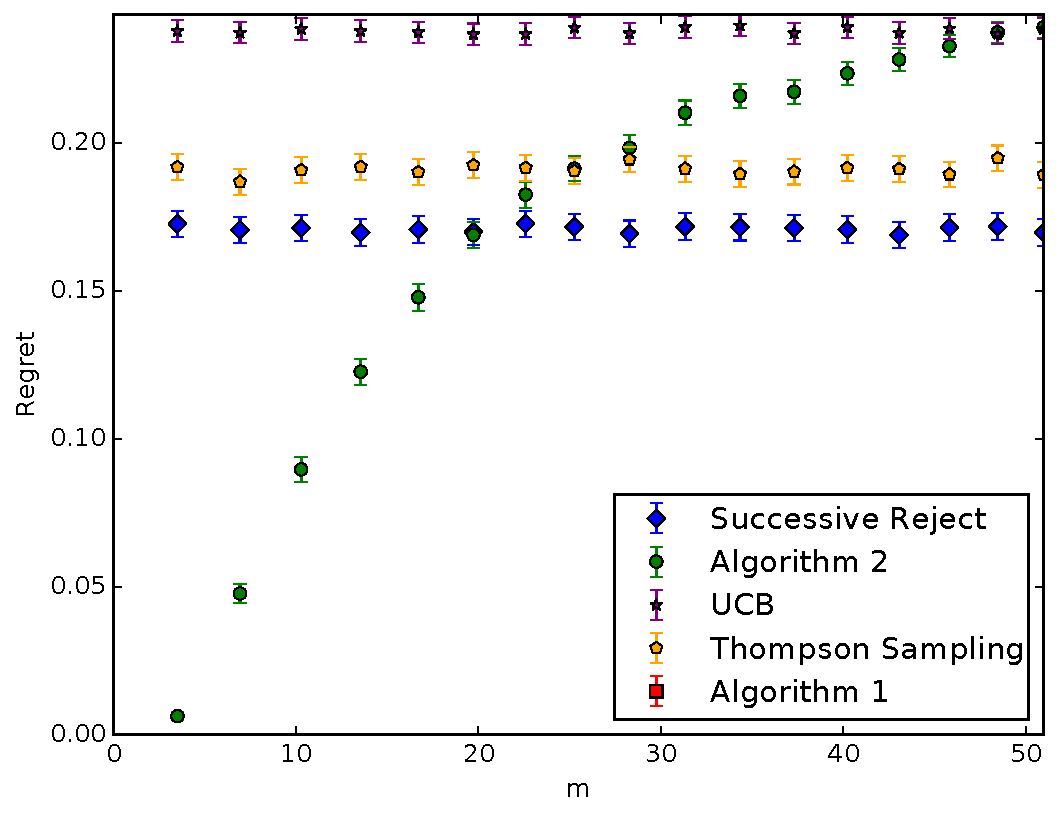
\includegraphics[width=\textwidth]{experiment4_20161023_2120.pdf}
    		\caption{Simple regret vs $m(\eta*)$ for fixed horizon $T=400$ and number of variables $N = 50$}
        \label{fig:simple_vs_m_general}
    \end{subfigure}\hfill
    \begin{subfigure}[t]{0.3\textwidth}
    		\centering
        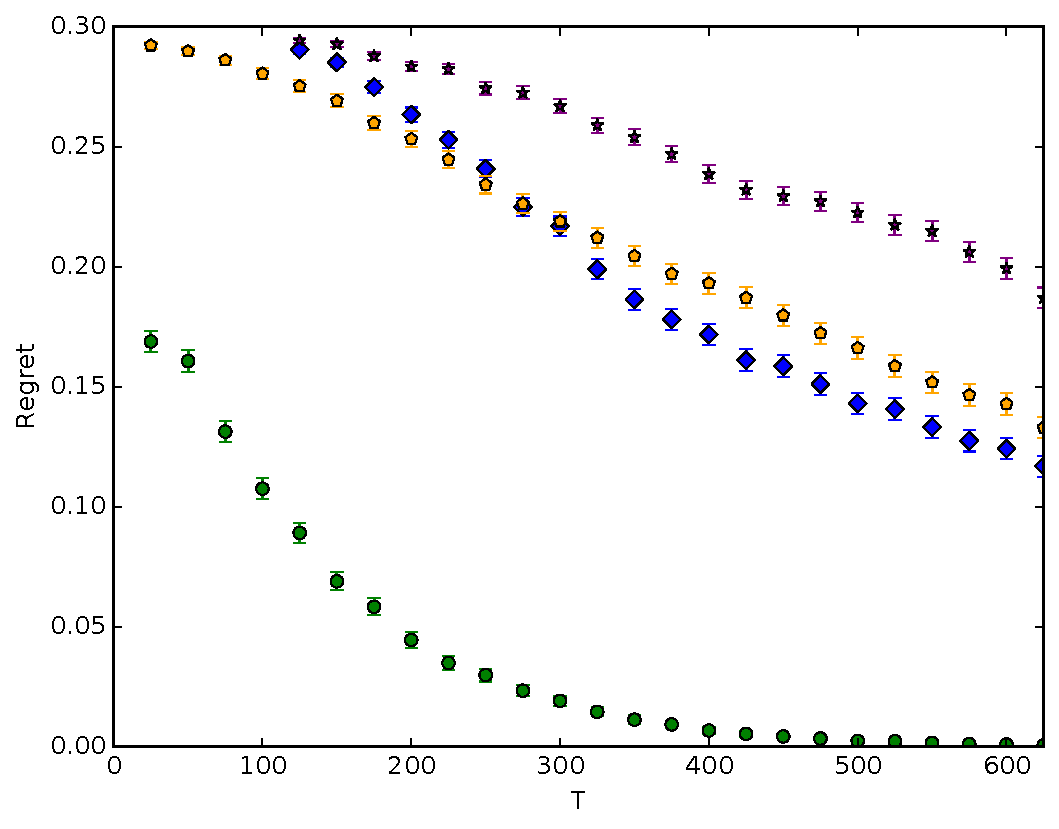
\includegraphics[width=\textwidth]{experiment7_20161020_1257.pdf}
    		\caption{Simple regret vs horizon, $T$, with $N = 50$ and $m(\eta*)=3.1$ }
        \label{fig:simple_vs_T_general}
    \end{subfigure}\hfill
    \begin{subfigure}[t]{0.3\textwidth}
    		\centering
    		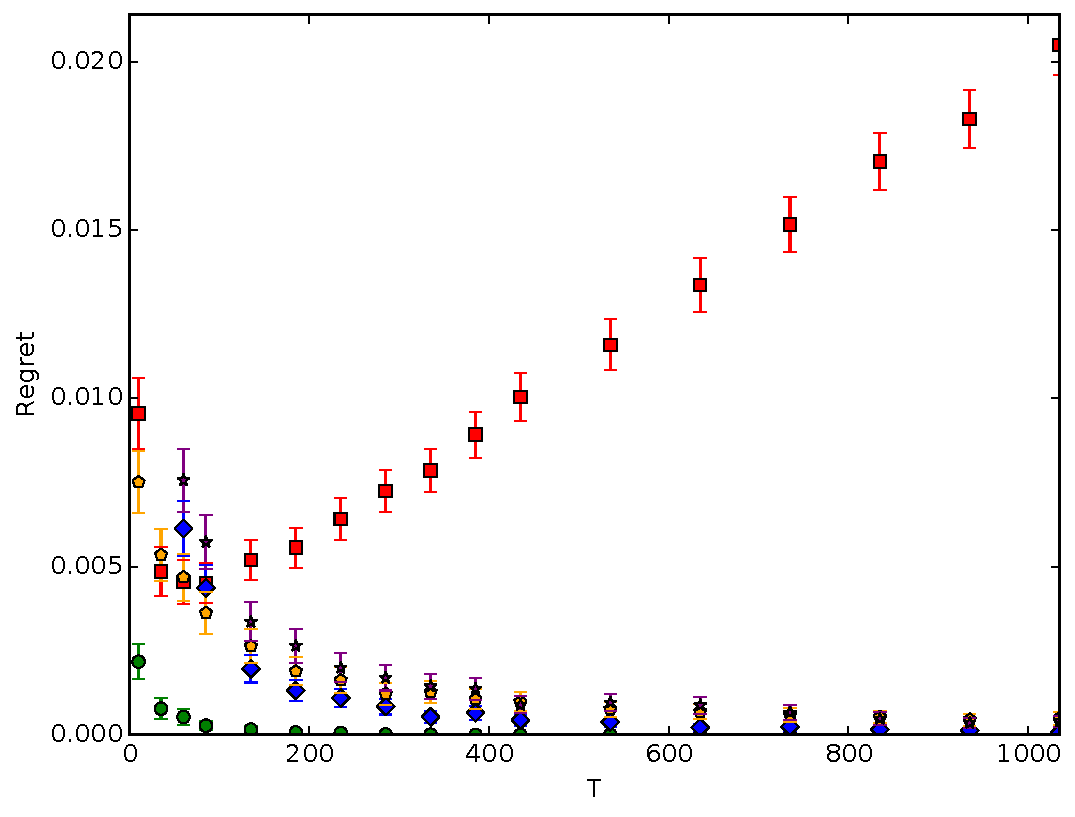
\includegraphics[width=\textwidth]{experiment5_20161023_2118.pdf}
    		\caption{Simple regret vs horizon, $T$, with $N = 21$, $m(\eta*)=4.3$ with no actions setting $Z$}
    		\label{fig:simple_vs_T_misspecified}
    \end{subfigure}
    \caption{Experimental results on the confounded graph in figure \ref{fig:parallel_confounded}}
    \label{fig:experiments_confounded}
\end{figure}

\end{block}
\end{column}

\begin{column}{\onecolwid} % The third column

%----------------------------------------------------------------------------------------
%	CONCLUSION
%----------------------------------------------------------------------------------------
\begin{block}{Conclusion}
\begin{itemize}
\item For parallel bandits we have an optimal algorithm (upto log factors) and simple measure of the difficulty of the problem $m(\vec{q})$.
\item For general graphs, $m(\eta) < N$ measures the difficulty of the problem. Finding an algorithm that only requires the causal graph and lower bounds for its simple regret in the general case is left as future work.
\end{itemize}
\end{block}

\begin{block}{Discussion \& Future work}

\begin{itemize}
\item The parallel bandit problem can be viewed as an instance of a time varying graph feedback problem, however the algorithms developed for this problem are not optimal for the parallel bandit.
\item Our algorithms only use the reward signal to estimate $\hat{\mu}_a$, not to inform which arms to sample. Making better use of the reward signal could substantially improve practical performance (but not minimax regret). 
\item Cumulative Regret

\item Generalize to consider causal bandit problems where the causal graph is partially or completely unknown. 

\end{itemize}





 

\end{block}



%%----------------------------------------------------------------------------------------
%%	ACKNOWLEDGEMENTS
%%----------------------------------------------------------------------------------------
%
%\setbeamercolor{block title}{fg=red,bg=white} % Change the block title color
%
%\begin{block}{Acknowledgements}
%
%\small{\rmfamily{Nam mollis tristique neque eu luctus. Suspendisse rutrum congue nisi sed convallis. Aenean id neque dolor. Pellentesque habitant morbi tristique senectus et netus et malesuada fames ac turpis egestas.}} \\
%
%\end{block}

%----------------------------------------------------------------------------------------
%	CONTACT INFORMATION
%----------------------------------------------------------------------------------------

\setbeamercolor{block alerted title}{fg=black,bg=norange} % Change the alert block title colors
\setbeamercolor{block alerted body}{fg=black,bg=white} % Change the alert block body colors

%\begin{alertblock}{Contact Information}
%
%\begin{itemize}
%\item Web: \href{http://www.university.edu/smithlab}{http://www.university.edu/smithlab}
%\item Email: \href{mailto:john@smith.com}{john@smith.com}
%\item Phone: +1 (000) 111 1111
%\end{itemize}
%
%\end{alertblock}



%----------------------------------------------------------------------------------------

\end{column} % End of the third column

\end{columns} % End of all the columns in the poster

\end{frame} % End of the enclosing frame

\end{document}
